\chapter{Web Server - Design of Experiment}
L'homework si pone l'obiettivo di valutare le performance del web server utilizzato per i precedenti lavori. In particolare lo studio è centrato sul \textit{response time}. Nel dettaglio bisogna studiare l'incidenza di due fattori sul tempo di risposta ricavando un'analisi ANOVA. I fattori di interesse sono:
\begin{itemize}
	\item \textbf{Page Type}, dimensione della risorsa da richiedere al server.
	\item \textbf{Intensità}, inteso come carico da applicare al sistema. 
\end{itemize}
Le performance possono essere valutate utilizzato le tecniche DOE (Design Of Experiment). 
\\Ogni misura effettuata inoltre deve essere ripetuta almeno 5 volte.

\section{Design}
I fattori utilizzati durante l'analisi, come già descritti, hanno un diverso numero di livelli. In particolare:
\begin{itemize}
	\item \textbf{Page Type}
	\begin{itemize}
		\item \textit{Small}        (S):  100 KB
		\item \textit{Small-Medium} (SM): 350 KB
		\item \textit{Medium-Large} (ML): 600 KB
		\item \textit{Large}        (L):  800KB
	\end{itemize}
	\item \textbf{Intensity}
	\begin{itemize}
		\item \textit{LOW}: 1500
		\item \textit{HIGH}: 4500
	\end{itemize}
\end{itemize}
I livelli del fattore \textit{Intensity} non sono scelti casualmente. Essi rappresentano una frazione della \textit{usable capacity} calcolata nel Capitolo 2. A tal proposito quindi il web server deve essere necessariamente identico a quello utilizzato per il \textit{\textbf{Capacity Test}}.
\\Un modello che può essere utilizzato per descrivere l'esperimento è il \textit{Two Factor Full Factor Design con Repliche}. poiché si hanno due fattori (con un numero arbitrario di livelli) e 5 ripetizioni per ogni misura. Per misura si intende la \textit{response time}.
\\Tale Design prevede di effettuare le misure per ogni combinazione tra i livelli dei due fattori; ogni misura deve poi essere ripetuta 5 volte. Posto $FACT_i$ come il numero di livelli del fattore $i$ e $R$ il numero di ripetizioni per ogni combinazione:
\begin{equation*}
	N = FACT_1 \times FACT_2 \times R = 2\times 4 \times 5 = 40
\end{equation*}
in cui $N$ è il numero di misure da effettuare.


\subsection{Client - JMeter}
Anche in questo caso per simulare le richieste con carico prefissato si utilizza il tool JMeter, ampiamente descritto in precedenza.
\\Per questo esperimento la configurazione è molto più semplice poiché bisogna porre solo una richiesta e un carico (che variano in relazione alla misura che si sta effettuando).
\\Ogni misura può durare anche solo 1min e il parametro di misurazione è \textit{elapsed} (ricavato stesso dal tool).
\\Per ogni misura il numero di richieste varia in relazione al carico, per cui il \textit{Response Time} può essere calcolato come la media tra tutti gli \textit{elapsed} che compaiono nelle misure.  
\begin{figure}[H]
	\centering
	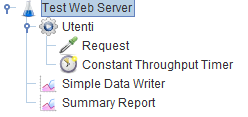
\includegraphics[width=0.4\textwidth]{img/hw4/jmeter.png}
	\caption{\textit{Configurazione di JMeter}}
\end{figure}
\vspace{0.5cm}
A questo punto per permettere di automatizzare il calcolo del \textit{response time}, i file di misurazione devono essere salvati con uno standard. Così facendo si può utilizzare MATLAB per calcolare il \textit{response time} (come media di \textit{elapsed}) in modo iterativo.
\\Ogni file viene dunque memorizzato nel seguente modo:
\begin{figure}[H]
	\centering
	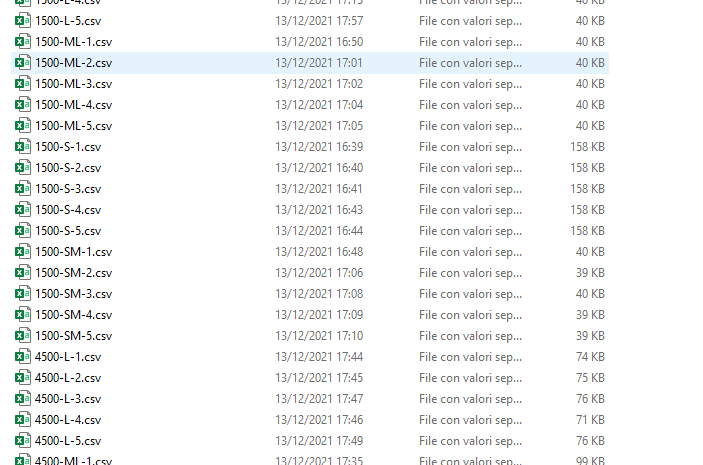
\includegraphics[width=0.7\textwidth]{img/hw4/file.png}
	\caption{\textit{Memorizzazione delle misure}}
\end{figure}
Il primo valore indica il carico (il livello del fattore \textit{intensity}), il secondo valore indica la risorsa (il livello del fattore \textit{page-type}), il terzo valore indica la ripetizione.
\\Dopo avere collezionato 40 file, con MATLAB si può automatizzare il calcolo:
\begin{minted}[framesep = 1mm,
	fontsize = \footnotesize,
	breaklines,
	]{MATLAB}
intensity = [1500 4500]; 
page_type = ["S", "SM", "ML", "L"];
N = 5;

resp_time = zeros(length(intensity),length(page_type), N);
factor_intensity = 1;
factor_page = 1;

for i=intensity
	for p=page_type
		for r=1:N
			path = strcat(num2str(i, '%d'),'-',p,'-',num2str(r, '%d'),'.csv');
			data = readtable(path);
			resp_time(factor_intensity,factor_page,r) = mean(table2array(data(:,2)));
		end
		factor_page = factor_page +1;
	end
	factor_intensity = factor_intensity +1;
	factor_page = 1;
end
\end{minted}
L'output è quindi una matrice tridimensionale che associa ad ogni combinazione di livelli e ad ogni ripetizione il corrispettivo valore del \textit{RT}.

\section{Analisi}
Il design oggetto di studio è un \textit{Two-factor Full Factorial Design con repliche}.
I fattori che lo interessano sono categorici, quindi possono assumere solo valori finiti. 
\\Utilizzando l'output prodotto durante la fase di design e di misurazione, si può costruire una tabella che racchiude tutti i tempi di risposta $y_{ijk}$.
\\La seguente tabella descrive i tempi medi di risposta ottenuti in funzione delle combinazioni dei fattori e delle repliche:
\begin{table}[H]
	\begin{center}
		\begin{tabular}{|c|c|c|c|c|}
			\hline
			Intensity & Small & Small-Medium & Meduim-Large & Large\\
			\hline
			\rule[-4mm]{0mm}{0.5cm}
			1500 & 5,2082 & 23,5713 & 42,0207 & 78,6531\\
			\rule[-4mm]{0mm}{0.5cm}
			& 5,7017 & 16,3747 & 32,3323 & 54,5792\\
			\rule[-4mm]{0mm}{0.5cm}
			& 5,4777 & 19,1214 & 32,6010 & 39,0433\\
			\rule[-4mm]{0mm}{0.5cm}
			& 5,9955 & 14,0742 & 36,6634 & 47,6427\\	
			\rule[-4mm]{0mm}{0.5cm}
			& 5,1065 & 16,8909 & 41,6693 & 55,1706\\ 
			\hline
			\rule[-0.5cm]{0mm}{0.5cm}
			4500 & 5,1412 & 15,4733 & 380,9312 & 552,1893\\
			\rule[-0.5cm]{0mm}{0.5cm}
			& 4,5569 & 18,6695 & 379,4760 & 538,0078\\
			\rule[-0.5cm]{0mm}{0.5cm}
			& 4,6629 & 23,1843 & 375,8755 & 539,3999\\
			\rule[-0.5cm]{0mm}{0.5cm}
			& 4,4400 & 21,3396 & 366,9233 & 575,0426\\	
			\rule[-0.5cm]{0mm}{0.5cm}
			& 4,3709 & 20,0086 & 368,5614 & 541,5188\\
			\hline
		\end{tabular}
	\end{center}
\label{experimental_data}
\end{table}
\subsection{Modello}
Sulla base della tabella Tab.\ref{experimental_data} si può costruire il modello che rappresenta il design scelto:
\begin{equation}
	y_{ijk} = \mu + \alpha_j + \beta_i + \gamma_{ij} + e_{ijk}
\end{equation}
in cui:
\begin{table}[H]
	\begin{center}
		\begin{tabularx}{\textwidth}{c|X|X}
			\textbf{Parametro} & \textbf{Significato} & \textbf{Dimensione}\\
			\hline
			$\mu$ & Media di tutte le misure & 1 \\
			\hline
			$ \alpha_j $ & Effetto del fattore \textit{Page-Type} & $a$ = Numero di livelli di \textit{Page-Type} \\
			\hline
			$ \beta_i $ & Effetto del fattore \textit{Intensisty} & $b$ = Numero di livelli di \textit{Intensisty} \\
			\hline
			$ \gamma_{ij} $ & Effetto dell'interazione dei due fattori & $b\times a$ = Numero di livelli di \textit{Intensisty} per il Numero di livelli di \textit{Page-Type}  \\
			\hline
			$ e_{ijk} $ & Errore di ogni misura & $b\times a\times r$ = Numero di livelli di \textit{Intensisty} per il Numero di livelli di \textit{Page-Type} per il Numero di Ripetizioni  \\
			
		\end{tabularx}
	\end{center}
\end{table}
Grazie alle conoscenze teoriche acquisite durante il corso, i parametri che descrivono il modello possono essere facilmente calcolati tramite uno script MATLAB.
\begin{minted}[framesep = 1mm,
	fontsize = \footnotesize,
	breaklines,
	]{MATLAB}
a = length(page_type);
b = length(intensity);
r = N;
%Parametri del modello
mu = 0;             %Media totale
alpha = zeros(1, a);%Effetto di PAGE TYPE
beta = zeros(1, b); %Effetto di INTENSITY
gamma = zeros(b, a);%Effetto dell'interazione
e = zeros(b, a, r); %Errore

%Calcoli
mu = 1/(a*b*r) * sum(resp_time,'all');
for j=1:a
	alpha(j) = sum(resp_time(:,j,:), 'all')/(r*b) - mu;
end
for i=1:b
	beta(i) = sum(resp_time(i,:,:), 'all')/(r*a) - mu;
end
for i=1:b
	for j=1:a
		gamma(i,j) = sum(resp_time(i,j,:),'all')/r - mu - alpha(j) - beta(i);
	end
end
for i=1:b
	for j=1:a
		for k=1:r
			e(i,j,k) = resp_time(i,j,k) - sum(resp_time(i,j,:),'all')/r;
		end
	end
end
\end{minted}
Esso fornisce come risultato:
\begin{figure}[H]
	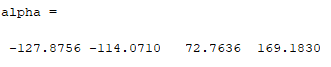
\includegraphics[width=0.5\textwidth]{img/hw4/alpha.png}
\end{figure}
\begin{figure}[H]
	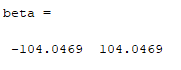
\includegraphics[width=0.3\textwidth]{img/hw4/beta.png}
\end{figure}
\begin{figure}[H]
	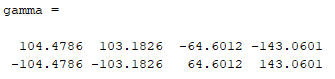
\includegraphics[width=0.5\textwidth]{img/hw4/gamma.png}
\end{figure}

\subsection{Importanza - Allocation of Variation}
L' \textit{importanza} di un fattore viene misurata in base alla porzione di \textbf{variazione totale} che esso riesce a spiegare.
\\Quest'ultima è espressa tramite la Sum of Squares Total o \textit{SST} la quale ci fornisce informazioni circa quanto i dati ottenuti si discostano dal loro valore medio.
\begin{equation}
	SST = \sum_{i = 1}^{b}\sum_{j = 1}^{a}\sum_{k = 1}^{r}{({y_{ijk}} - \mu)^2}
\end{equation}
con $a$ la dimensione di $\alpha$, $b$ la dimensione di $\beta$ e $r$ numero di ripetizioni.
\\In particolare la variazione totale può essere anche vista come somma delle variazioni spiegate dai fattori, dalle loro interazioni e dall'errore commesso:
\begin{equation*}
	SST = SSA + SSB + SSAB + SSE
\end{equation*}
La percentuale di variazione spiegata dal fattore A ad esempio è: 
\begin{equation*}
	A = \dfrac{SSA}{SST} \times 100
\end{equation*}
Queste informazioni possono essere agevolmente ottenute in \textit{JMP}, operando sulla tabella che caratterizza il design in questione, analizzando le sezioni:
\begin{enumerate}
	\item \textit{Analisi della varianza}
	\item \textit{Test degli effetti}
\end{enumerate}
\subsubsection{Caso di Studio}
\begin{figure}[H]
	\subfigure{	
		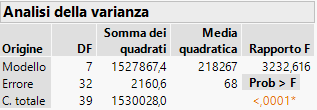
\includegraphics[width=0.50\textwidth]{img/hw4/AnalisiVarianza.png}}
	\subfigure{	
		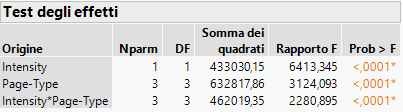
\includegraphics[width=0.62\textwidth]{img/hw4/TestEffetti.png}}
	\caption{\textit{Sum of Squares in JMP}}
\end{figure}
\begin{table*}[h]
	\begin{center}
		\begin{tabular}{|c|c|c|}
			\hline
			Component &  Sum of Squares & \% Variation\\
			 \hline
			    $y-\overline{y}_{...}$ & 1530028,0		   & 100\\
			 \rule[-4mm]{0mm}{0.5cm}
			 Intensity (CTTs) 		   &433030,15		   & 28,30\\
			 \rule[-4mm]{0mm}{0.5cm}
			 Page-Types 		   &632817,86		   & 41,36\\
			 \rule[-4mm]{0mm}{0.5cm}
			 Interactions		   &462019,35		   & 30,20\\
			 \rule[-4mm]{0mm}{0.5cm}
			 Errors 		   &2160,6		   & 0,14\\
			\hline
		\end{tabular}
	\end{center}
\end{table*}
Osservando i risultati ottenuti si nota che la percentuale maggiore di variazione la spiega il fattore \textit{Page Types}, con il 41,36\% della totale, seguito da \textit{Interazioni} e \textit{Intensità del carico} che ne spiegano una percentuale più o meno simile (rispettivamente 28,30\% e 30,20\%). Il restante 0,14\% è attribuita all'errore sperimentale.
\\Gli stessi risultati possono essere tranquillamente raggiunti anche con uno script MATLAB che sfrutta il modello precedentemente calcolato.
\begin{minted}[framesep = 1mm,
	fontsize = \footnotesize,
	breaklines,
	]{MATLAB}
SSY = sum(resp_time(:,:,:).^2, 'all');
SS0 = a*b*r*mu*mu;
SSA = b*r*sum(alpha.^2);
SSB = a*r*sum(beta.^2);
SSAB = r*sum(gamma.^2, 'all');
SSE = sum(e.^2, 'all');
SST = SSY - SS0;
IMPORTANZA_PAGE_TYPE = SSA/SST;
IMPORTANZA_INTENSITY = SSB/SST;
IMPORTANZA_INTERACTION = SSAB/SST;
IMPORTANZA_ERRORE = SSE/SST;
\end{minted}
Dunque i risultati di JMP possono essere integrati con questi ottenuti tramite lo script MATLAB, racchiudendo il tutto in un'unica tabella:
\begin{table}[H]
	\begin{center}
		\begin{tabular}{|c|l|c|c|l|}
			\hline
		\textbf{Component} & \textbf{Sum of Squares} & \textbf{\% Variation} & \textbf{DF} & \textbf{Mean Square} \\
		\hline
		$y$ & $SSY=2236968$ & & $40$ &  \\
		$\bar{y}$ & $SS0 = 706940$ & & $1$ & \\
		$y-\overline{y}_{...}$ & $SST = 1530027$ & $100$ & $39$ & \\
		Page-Type & $SSA = 632817$ & $41,36$ & $3$ & $MSA = 210939$ \\
		Intensity & $SSB = 433030$ & $28,30$ & $1$ & $MSB = 433030$ \\
		Interaction & $SSAB = 462019$ & $30,20$ & $3$ & $MSAB = 154006$ \\
		$e$ & $SSE = 2160$ & $0,14$ & $32$ & $MSE = 67,52$ \\
		\hline
		\end{tabular}
	\end{center}
\end{table}
Tuttavia l'importanza non è un concetto statistico, dunque si necessita la valutazione di un altro parametro che invece lo è, la significatività.
Difatti può accadere che un fattore importante non sia significativo.
\subsection{Significatività - Analysis of Variance}
La \textit{significatività} di un fattore, come precedentemente specificato, è un concetto statistico il quale esplicita il contributo che spiega quel fattore rispetto a quello relativo all'errore.
\\Se un fattore è significativo, ripetendo l'esperimento, con elevata probabilità (associata al livello di significatività) esso influenzerà sempre allo stesso modo l'output, dimostrando che quindi quei risultati non sono dettati dal caso.
\\
\\Gli ANOVA (Analysis of Variance) tests permettono di verificare la significatività dei fattori di un esperimento. Al pari dei test d'ipotesi discussi nel capitolo precedente, anch'essi si basano su delle assunzioni tra cui:
\begin{itemize}
	\item \textbf{Normalità dei residui}.
	\item \textbf{Omoschedasticità}.
\end{itemize}
In base a se queste due condizioni sono verificate o meno, verrà utilizzato un particolare test. Nella seguente tabella sono sintetizzate tutte le combinazioni tra le varie condizioni con il relativo test da applicare:
\begin{figure}[H]
	\centering
	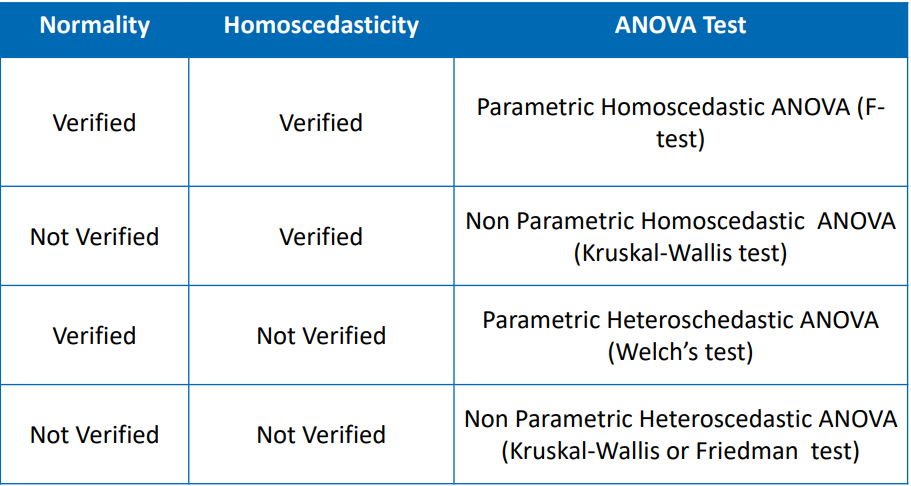
\includegraphics[width=0.8\textwidth]{img/hw4/ANOVATests.png}
	\caption{\textit{Tabella ANOVA tests}}
	\label{table}
\end{figure}
\subsubsection{Caso di Studio - Check Normalità}
Per poter decidere quale test utilizzare per studiare la significatività di \textit{Intensity} e \textit{Page-Types} si deve quindi verificare innanzitutto se i residui (risposta osservata - valore previsto) provengono da una distribuzione normale.
\\JMP permette di ricavare la colonna dei residui automaticamente a partire da livelli - ripetizioni e output. In seguito alla generazione si può effettuare un plot della distribuzione, in particolare il \textit{normal quantile plot}
\begin{figure}[H]
	\centering
	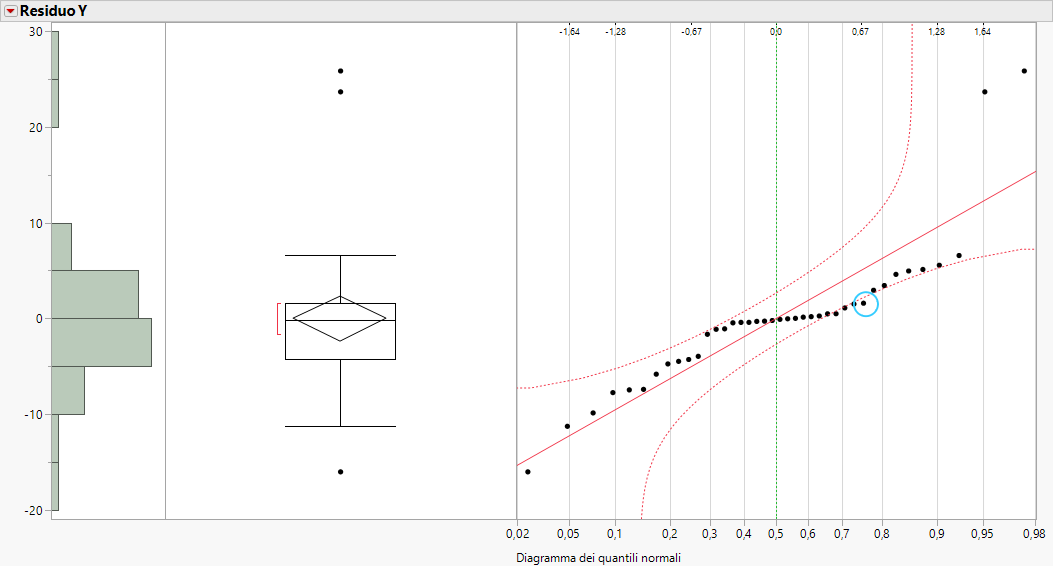
\includegraphics[width=0.8\textwidth]{img/hw4/qqplot_res.png}
	\caption{\textit{Normal quantile plot JMP}}
\end{figure}
il quale non è altro che il q-qplot già discusso per la workload characterization.
\\Si assume che la distribuzione considerata non è normale se anche uno solo dei residui esce al di fuori delle bande di confidenza (tratteggiate e in rosso). In questo caso si verifica con evidenza proprio questa situazione, dunque \textbf{la normalità non è verificata}.
\\Si può validare ulteriormente tale assunzione attraverso il test statistico di \textit{Shapiro-Wilk}, tenendo conto del fatto che se dovesse fornire un risultato diverso da quello del test visivo, in ogni caso sarà l'esito di quest'ultimo (del test visivo) ad essere preferito.
\begin{figure}[H]
	\centering
	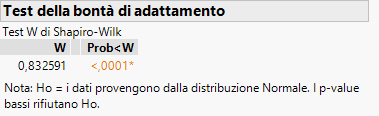
\includegraphics[width=0.5\textwidth]{img/hw4/shapiro_wilch.png}
	\caption{\textit{Test di Shapiro Wilk}}
\end{figure}
Il test restituisce un \textit{P-value} basso, dunque l'ipotesi nulla è stata rigettata ad ulteriore conferma della non normalità della nostra distribuzione.
\subsubsection{Caso di Studio - Check Omoschedasticità}
L'uguaglianza delle varianze viene valutata esclusivamente per ogni fattore. Lo si fa prendendo in considerazione uno dei seguenti test:
\begin{enumerate}
	\item \textit{Bartlett}
	\item \textit{Levene}
	\item \textit{O'Brien}
	\item \textit{Brown-Forsythe}
\end{enumerate}
i cui risultati sono agevolmente forniti da JMP.
\begin{figure}[H]
	\subfigure{	
		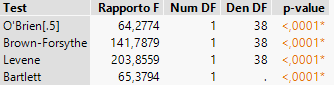
\includegraphics[width=0.50\textwidth]{img/hw4/omo_i.png}}
	\subfigure{	
		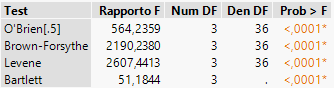
\includegraphics[width=0.50\textwidth]{img/hw4/omo_pt.png}}
	\caption{\textit{Test omoschedasticità Intensity e Page Type}}
\end{figure}
Indipendentemente dal test scelto, per entrambi i fattori \textbf{non vale l'ipotesi di omoschedasticità}. Difatti il \textit{P-value} basso ci suggerisce che l'ipotesi nulla è stata rigettata.
\subsubsection{Caso di Studio - Check Significatività fattori}
Considerando la \ref{table} ci si trova nel caso 4, con normalità e omoschedasticità non verificate. I test da poter applicare fanno parte degli ANOVA non parametrici eteroschedastici: \textbf{Kruskal-Wallis test o Friedman test}.
Prendendo in considerazione il primo (sarebbe stato lo stesso anche se avessimo verificato l'omoschedasticità):
\begin{figure}[H]
	\centering
	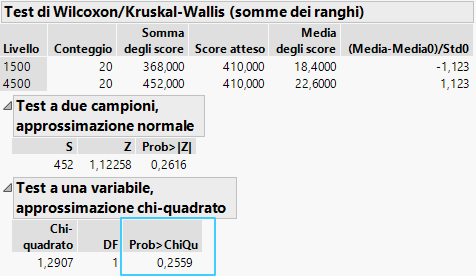
\includegraphics[width=0.6\textwidth]{img/hw4/KW_i.png}
	\caption{\textit{Test di Kruskal-Wallis Intensity}}
\end{figure}
Il valore alto (in nero) del P-value indica che il fattore Intensity non è risultato significativo ai fini dei tempi di risposta.
\begin{figure}[H]
	\centering
	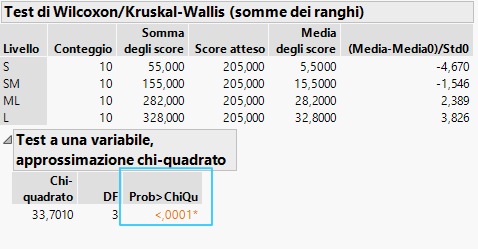
\includegraphics[width=0.6\textwidth]{img/hw4/KW_pt.png}
	\caption{\textit{Test di Kruskal-Wallis Page-Type}}
\end{figure}
Il P-value in questo caso assume un valore abbastanza piccolo (in arancione), dunque il fattore Page-Type oltre ad essere quello più importante risulta anche l'unico fattore significativo per l'output.
\\Ciò si poteva intuire perché, osservando i dati in Tab.\ref{experimental_data}, il tempo di risposta per pagine Small e Small-Medium è molto simile indipendentemente dal carico. Non appena la dimensione varia, e quindi il tipo di pagina, il tempo di risposta aumenta/varia e i tempi di risposta associati ai due carichi sono completamente diversi. 